%%%%%%%%%%%%%%%%%%%%%%%%%%%%%%%%%%%%%%%%%%%%%%%%%%%%%%%%%%%%%%%%%%%%%%%%%%%%%
%	e-Yantra, IIT-Bombay

%	Document Author: Aditya Kumar and Pritish Saluke

%%%%%%%%%%%%%%%%%%%%%%%%%%%%%%%%%%%%%%%%%%%%%%%%%%%%%%%%%%%%%%%%%%%%%%%%%%%%%

\documentclass[11pt,a4paper]{article}
\usepackage{listings}
\usepackage{url}
\usepackage{graphicx}
\title{Interrupt using SPI, I2C and UART}
\author{e-Yantra Team}
\date{\today}

\begin{document}
	\maketitle
	\newpage
	\tableofcontents
	\newpage
	\section{Objective}
	In this tutorial we will learn interrupt using SPI, I2C and UART protocol.
	\section{Prerequisites}
	\begin{itemize}
		\item Python programming skills(Concept of threading)
		\item Knowledge about Arduino
	\end{itemize}
	\section{Hardware Requirement}
		\begin{enumerate}
			\item Raspberry Pi (I will be using Version 2 Model B+)
			\item Power adapter
			\item Connecting wires
			\item Arduino
			\item Resistor (3.3K)
			\item Push Button
		\end{enumerate}
	\section{Software Requirement}
	\begin{enumerate}
		\item PyScripter (version 2.7 or above)
		\item Mobaxterm (for windows users)
	\end{enumerate}
	\newpage
	\section{Theory and Description}
	\textbf{Interrupt}
	\newline
	 An Interrupt is a signal generated by some event external to CPU, which causes the CPU to stop what it is doing and go to separate piece of code known as ISR for execution. When the execution of ISR completes it starts main program from where it left. \\
	 \flushleft
	 \textbf{Types of Interrupt} \\
	 \begin{itemize}
	 	\item{Hardware Interrupt} \\
	 	Hardware interrupts are used by devices to communicate that they require attention from the operating system.These interrputs are requested by external peripherals such as keyboard, moving the moving trigger.
	 	\item {Software Interrupt} \\
	 	A software interrupt is a type of interrupt that is caused either by a special instruction in the instruction set or by an exceptional condition in the processor itself. A software interrupt is invoked by software, unlike a hardware interrupt, and is considered one of the ways to communicate with the kernel or to invoke system calls, especially during error or exception handling.
	 \end{itemize}
	 \textbf{Interrupt through UART}\\
	 
	 Whenever CPU receives interrupt request from external device using UART. Control goes to receives data from devices. After that control returns to its main program execution.\\
	 
	 \textbf{Interrupt through I2C protocol}\\
	 
	 The Inter-integrated Circuit (I2C) Protocol is a protocol intended to allow multiple “slave” digital integrated circuits (“chips”) to communicate with one or more “master” chips. I2C requires a mere two wires, like asynchronous serial, but those two wires can support up to 1008 slave devices. 
	  I2C can support a multi-master system, allowing more than one master to communicate with all devices on the bus (although the master devices can’t talk to each other over the bus and must take turns using the bus lines). Whenever CPU receives interrupt request from external device using I2C protocol.Control goes to receives data from devices. After that control returns to its main program execution.\\
	  
	  \textbf{Interrupt through SPI Protocol} \\
	  
	  SPI is a single-master communication protocol. This means that one central device initiates all the communications with the slaves. When the SPI master wishes to send data to a slave and/or request information from it, it selects slave by pulling the corresponding SS line low and it activates the clock signal at a clock frequency usable by the master and the slave. The master generates information onto MOSI line while it samples the MISO line.\newline
	  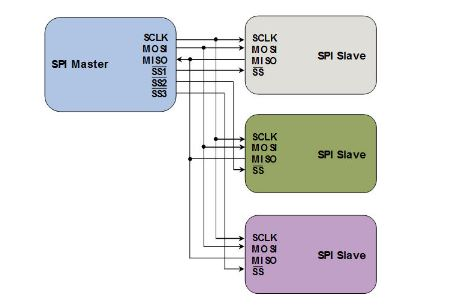
\includegraphics[scale=0.8]{SPI.jpg}
	  \vspace{5mm}
	  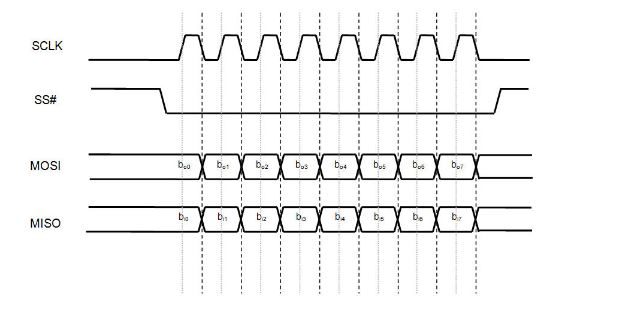
\includegraphics[scale=0.7]{SPI1.jpg}
	\section{Experiment}
	
	\subsection{External Interrupt}
	In this experiment we will detect falling edge of GPIO pins. Gpio pin is connected to the switch. So, when switch is pressed, it is detected and ISR is called.\\
	\centering
	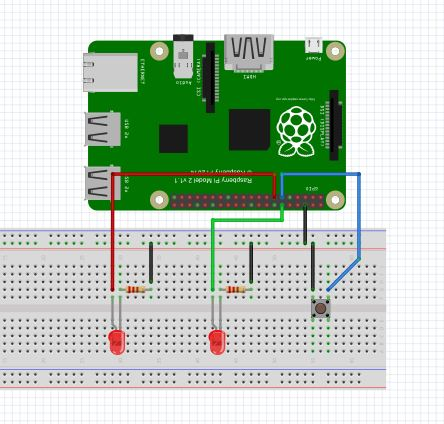
\includegraphics[scale = 0.6]{switch_interrupt}
	\flushleft
	\textbf{Code}
	\vspace{0.3cm}
	\lstinputlisting[language=Python]{external_GPIO_interrupt.py}
	\newpage
	\textbf{Same experiment is done by threading. Code for it is given below.} \\
	\vspace{5mm}
	
	\textbf{Code}
	\vspace{0.3cm}
	\lstinputlisting[language=Python]{external_interrupt_thread.py}
	
	\subsection{Communication between RPi and Android device using UART protocol}  
	In this experiment, main program in python remain in execution when we send data from android device. It does does wait for data. When data receive it prints it on the screen.
	\newpage
	Connections of Bluetooth modules is as follows:\\
	\vspace{5mm}
	\begin{figure}
		\centering
		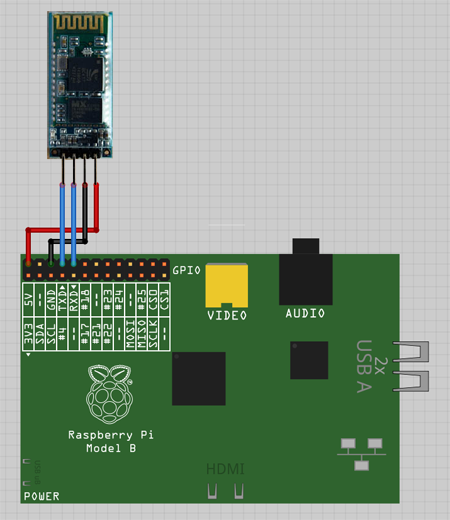
\includegraphics[scale = 0.4]{bluetooth.png}
	\end{figure}
	\textbf{Code}
	\vspace{0.3cm}
	\lstinputlisting[language=Python]{serial_interrupt_blue.py} 
	
	\subsection{Interrupt using SPI Protocol}
	In this experiment, Arduino interrupts RPi using SPI protocol. On Arduino board we have intefaced a switch and interrupt occurs when switch is pressed. In Python we make a thread polling the status of switch continuousally and in another thread our main program continues.\\
	\vspace{5mm}
	\textbf{Connections:}\\
	\vspace{5mm}
	\centering
	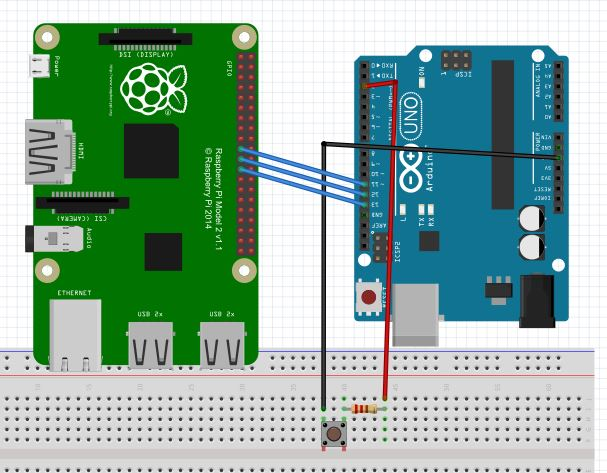
\includegraphics[scale= 0.4]{rpi_with_arduino_spi.jpg}
	\vspace{5mm}
	\flushleft
	\textbf{Code}
	\vspace{5mm}
	\lstinputlisting[language=Python]{spi_interrupt.py}
	\newpage
	\textbf{Arduino UNO Code:}
	\vspace{5mm}
	\lstinputlisting{spi_slave.ino}
	\subsection{Interrupt using I2C Protocol} 
	In this experiment, Arduino interrupts RPi using I2C protocol. On arduino board we have intefaced a switch and interrupt occurs when switch is pressed. In Python we make a thread polling the status of switch continuousally and in another thread our main program continues.. \\
	\vspace{5mm}
	\textbf{Connections are as shown below:}\\
	\vspace{5mm}
	\centering
	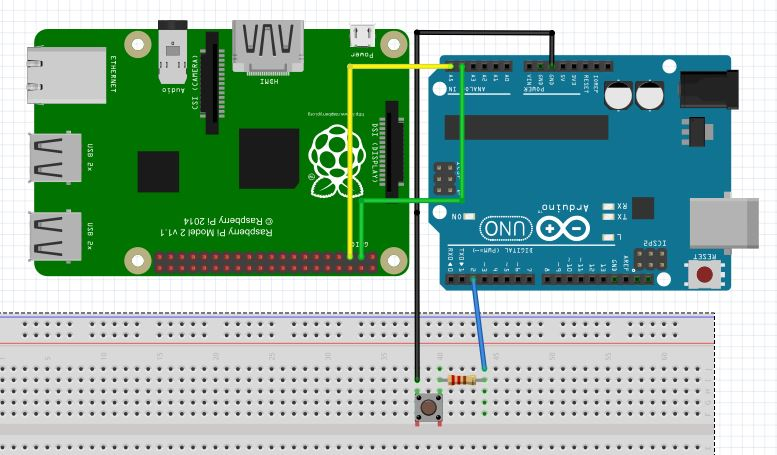
\includegraphics[scale=0.5]{rpi_with_arduino.jpg}
	\flushleft
	\vspace{5mm}	
	\textbf{Code}
	\vspace{5mm}
	\lstinputlisting[language=Python]{i2c_interrupt.py}
	\vspace{5mm}
	\textbf{Arduino UNO Code:}
	\vspace{5mm}
	\lstinputlisting{i2c_switch_press.ino}
	\section{Exercise}
	\begin{enumerate}
			\item Interface a dc motor through L293D motor driver IC using hardware PWM pins(GPIO 18 or IC pin 12) on RPi.
	\end{enumerate}
	
	\section{Appendix}
	\subsection{PIN Diagram}
	\textbf{Arduino Board Pins}
	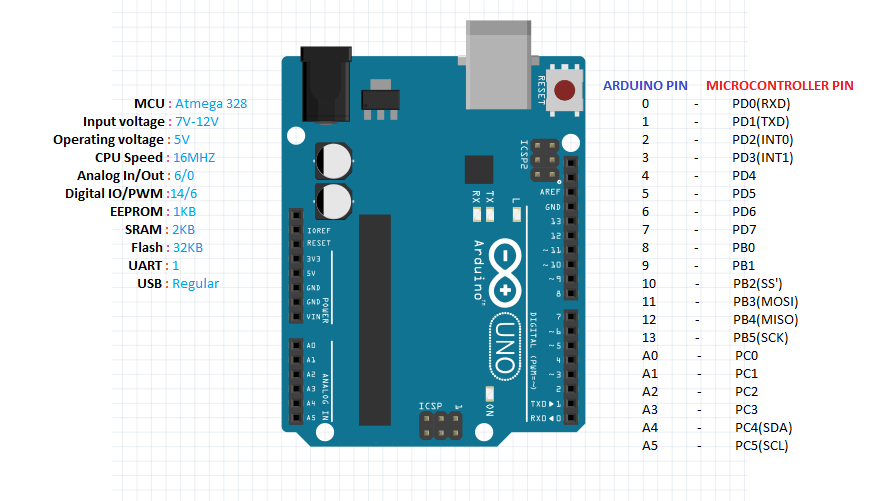
\includegraphics[scale=0.7]{arduino.png}  
	\newline
	\subsection{Datasheets}
	\textbf{ATMEGA328} \\
	\url{www.mouser.com/pdfdocs/Gravitech_ATMEGA328_datasheet.pdf}\\
	
	\section{References}
	\begin{enumerate}
		\item https://www.techopedia.com/definition/22195/software-interrupt
		\item http://www.byteparadigm.com/applications/introduction-to-i2c-and-spi-protocols/
	\end{enumerate}
	
\end{document}



